\vspace{0pt}
\lettrine[lines=2, findent=3pt,nindent=0pt]{M}{etrology}, as the science of measuring, has played an essential role for the development of the technology as we know it today.
It studies several aspects of the estimation process, such as which strategy to follow in order to improve the precision of an estimation.
One of the most important figure of merit in this context is the achievable precision for a given system, independently of the strategy.
We will show how to characterize it in the subsequents sections.
And we will show as well different strategies to achieve the desired results.
The metrology science also covers from the design aspects of a precise measuring device, until the most basic concepts of nature which lead in ultimate instance to the better understanding of the whole process.

In this sense, with the discovery of the Quantum Physics and the development of Quantum Mechanics, new doors for advances in metrology were open on the earlies decades of the 19th century.
Later on, the Quantum Theory lead to the so-called field of Quantum Information which merges the notions of the theory of information and computer science, among others subfields, with the quantum mechanics.
The role of the so-named entanglement, an exclusive feature of Quantum Mechanics, is essential in this context.
Its complete understanding has integrated efforts of many researches world wide.
Said this, the entanglement also is in the center of theoretical concepts included in Quantum Metrology.

On the other hand and with the aim of interpreting raw data, there are the statistics, without which many descriptions of the actual and past physical findings would lack of the rigorous interpretation needed for the complexity of data samples.



\subsection{Background on statistics and theory of estimation}
The main mathematical tools used by the metrology science belong to statistics.
Moreover we are also interested on estimation theory.
The statistics main characteristic is that makes the raw data under consideration comprehensible.
The data can be anything, from a set of different heights of a basketball team, to the outcomes of a coin toss or the ages of a hundred students or even the outcomes of a thousand times repeated measurement of the electric field at some spatial point.
The aim of this section is to give the reader sufficient material to follow this thesis and make it comprehensible from the beginning.

\subsubsection{Data sample, average, variance and central moments}

As we mentioned above, everything in statistics starts with a data set.
A dataset is defined as a set of values, we will restrict ourselves to quantitative values, representing some physical quantity.
So in our framework the set can be written as $X=\{x_i\}_{i=1}^M$, where all different $M$ values are collected.

With this data at hand, we are able to compute the \emph{arithmetic average} of the set, namely $\text{E}[X] := \frac{1}{M}\sum_{i=1}^M x_i$.
There are other types of averages such as the geometric mean, the root mean square or the harmonic mean, see reef. [XXX].
For us will be enough with the arithmetic average.

The second quantity one can compute is how spread the data is.
Namely the \emph{variance}, which can be defined easily as $\text{V}[X] := \text{E}[(X- \text{E}[X])^2]$, where $X$ can be seen as a vector and when subtracting the scalar $\text{E}[X]$ and $X^2$ stands for the elements wise squared of $X$, namely $X^2 := \{x_i^2\}_{i=1}^M$.
Similarly can be done for higher orders.
The variance is also a well known quantity on many fields of science.
It can also be written alternatively as $\text{V}[X] = \text{E}[X^2]- \text{E}[X]^2$.
The definition of the \emph{standard deviation} follows directly from the variance, $\sigma_{X}=\sqrt{\text{V}[X]}$.
Many quantities on statistics require operations like the one above.

At this point, let us illustrate thees quantities with an example.
It will also help us for introducing another concept.
Let us have the outcomes of, let us say, measurements of the heights of 18 trees.
Let us have those heights as integer values and in meters, see Tab. [XXX].
Then, the average height of the set is simply $\text{E}[X] = \frac{1}{18}\sum_{i=1}^{18} x_i = 6\text{m}$. Now let us see what happens with the variance, $\text{V}[X]=\frac{1}{18}\sum_{i=1}^{18}x_i^2 - 6^2 = 5.5\bar{5}\text{m}^2$.
Using now the standard deviation one can say about the original distribution that most values are around 6m with a deviation of 2.357m. Of course, some values are outside this range, but nevertheless the description is quite accurate, note that 12 values from 18 are inside the range $6\text{m}\pm2.357\text{m}$.

\begin{table}
\begin{center}
\begin{tabular}{| l | c | c | c | c | c | c | c | c | c | c | c | c | c | c | c | c | c | c | }
  \hline
  Tree \# & 1 & 2 & 3 & 4 & 5 & 6 & 7 & 8 & 9 & 10 &  11 &  12 &  13 &  14 &  15 &  16 &  17 &  18
  \\ \hline
  Heights (m) & 6 &  7 &  5 &  7 &  2 & 11 &  7 &  4 &  7 &  2 &  7 &  7 &  5 &  5 &  5 &  8 &  3 & 10 \\ \hline
\end{tabular}
\end{center}
\caption{A set of values for the heights of 18 trees. All measurements were rounded to integers for simplicity.}
\end{table}

Can we simplify the way we represent the data?
One may notice that the value 7m is repeated 6 times, as the value 5m is 4 times and so on.
For that we will introduce the distribution function $p_i$, which in this case is for discrete values of the outcomes but which can be generalized for continuous variables.
This function takes the value of how many times the outcome $i$ has appeared on the data sample.
Let us plot the distribution function on what is usually referred as \emph{histogram}.

\begin{figure}
  \centering
  \subfloat{
    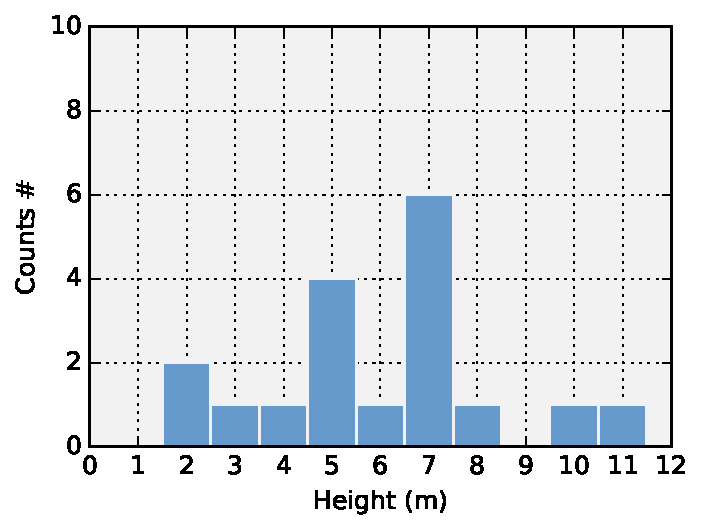
\includegraphics[width=0.4854015\textwidth]{img/plots/BG_hist_bin_1.pdf}}
  \hfill
  \subfloat{
    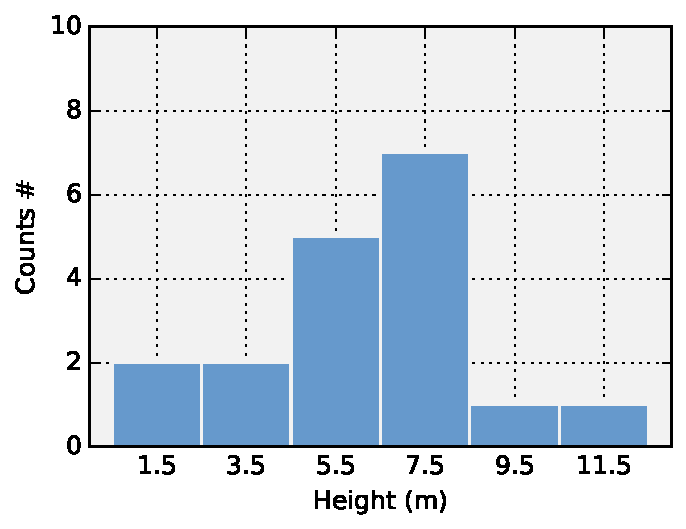
\includegraphics[width=0.475\textwidth]{img/plots/BG_hist_bin_2.pdf}}
  \caption{\baselineskip=14pt (a) $p_i$ for different values of $i$. All bars have width as 1, so it is drawn how many times each data value appears on the data sample.
  The width of the bars is called \emph{bin}, and it can change so the bars would represent a wider range of values. (b) Yo can see the same data represented in this case by a histogram with the bin size equal to 2. To produce this histogram we have summed 2 adjacent $p_i$ values starting from $p_1+p_2$, $p_3+p_4$ and so on.
  Those new bars we have chosen to represent a value in between, for instance $(3+4)/2=3.5$ and so on.}
\end{figure}

Now some question arises immediately:
How this is fully connected with the previous picture?
How can one compute the average and other interesting quantities?
The answer is simple but it has to be considered carefully.
First of all, notice that $p_i$ is defined for all the natural numbers including zero, see that in the example of the trees $p_9$ equals zero, so it can be extended for other heights too setting them to zero.
This will depend on the physical property that our data sample represents but in this case it is the height of some trees, so the values cannot be negative.
Second, notice that the sum of all the repetitions, all the values of $p_i$, is exactly 18 the number of data samples in the set.
So we have that $M = \sum_{i=0}^{\infty} p_i$.
Now we can formulate the ensemble average as $\text{E}[X]=\sum_{i=0}^{\infty} p_i i / \sum_{j=0}^{\infty} p_j$. The variance and with this the standard deviation immediately follow this approach.
It is convenient to notice that the total measurement outcomes has not contribute anything but to normalize the quantities.

We can now without losing generality redefine the distribution function to be the number of repetitions corresponding to the variable divided by the total outcomes, in this case $M$.
It would have the same properties of a probability distribution function (PDF).
For instance, now we have that the sum of all $p_i$-s equal to one, $\sum_{i=0}^\infty p_i = 1$, and the average is directly obtained by computing  $\text{E}[X] = \sum_{i=0}^\infty p_i i$.
This is the approach we will follow to represent data samples.
The variance and other quantities also are simpler in this way.

\subsubsection{Probabilities and frecuentist vs. bayesian approach}

The trivial values to compute from the data

We can estimate the average height of the trees of that forest.

histogram

estimator

MLH

CLT




\subsection{Quantum Mechanics}
The ubiquitous probabilistic nature of quantum mechanics is reflected on each corner of the field.
This \emph{ambiguity} of a system been quantum is exploited by many recent technologies.

The state

product states

Entanglement

Evolution

Unitary evolution

Markov

Limblad

Measurements

\subsection{Quantum Metrology}

Histograms of quantum states

Merging the probabilistic features of quantum mechanics with the estimation theory is not tibial.

The figure of merit for this purpose is the so-called Quantum Fisher Information.
